\section{Introduction}
\label{sec:maggie_introduction}

\newcommand\rvir{r_{\rm vir}}
\newcommand\vvir{v_{\rm vir}}
\newcommand\pps{\emph{pps}}

We showed in the previous chapter that the very popular grouping algorithm
should have its two linking lengths optimized, and that this depends on the
scientific goal of the group catalog obtained. With these limitations, it is
clear why Bayesian methods appeared. Indeed, with our knowledge of the galaxy
formation and evolution processes, it is possible to constrain better the
galaxy grouping. With the FoF algorithm, galaxies are selected in a pure
geometrical way, and their formation history doesn't matter in this selection,
since only the over-density is relevant. With Bayesian algorithms, it is
possible to combine geometrical and physical approaches. The history of
galaxies is available by their observable properties such as luminosity,
stellar mass, morphology and is used to assign galaxies to a group, in
complement of the geometrical information from the density. In particular, a
galaxy can be rejected of a group selected by density criterion if its
properties don't reflect the history it would have inside this group.

We already described Bayesian algorithms in
\bartrefchapter{galaxy_group_algorithms}, for example \citet{Yang+07} or
\citet{DominguezRomero+12}, where similar spatial methods to the FoF are
adopted, with priors on the density profile of galaxies inside halos to
constrain the assignment. But because of observational uncertainties, model
divergences, various incompletenesses\ldots, the extraction of groups from
observational data will always be affected by these problems, and the galaxy
environment polluted by interlopers, creating biases in group characteristics.
This leads to the blurring of the modulation of galaxy properties with their
environment and of our understanding of intra-groups physical processes.

Recently, with the improvement of computer performances in terms of memory and
CPU power, it becomes possible to include many priors in the computation, and
to use the most computer-intensive applications of statistics. Since
interlopers will still be problematic, the new powerful computer era allows for
probabilistic membership of galaxies in groups. Systematic errors in galaxy
surveys can be reduced or integrated in the grouping by probabilities. For
example, \citet{Liu+08} used a probabilistic FoF in a galaxy survey with
photometric redshifts to avoid the uncertainties inherent to this method.
\citet{DominguezRomero+12} also used ``responsibilities'' to improve the
assignment of galaxies to groups and reduce the effect of interlopers on the
observable properties of groups. In \citet{Rykoff+14}, galaxies have their
probabilities based on the group richness estimations.

It seems that using probabilities to describe the membership inside galaxy
groups will be inevitable, because of the systematic errors and biases presents
in the actual and future galaxy surveys. In particular, the modulation of the
galaxy properties with their environment that we want to extract from galaxy
group catalogues should be less biased by interlopers if we use probabilities
as weights. Indeed, interlopers, even if they are still present in the group
membership, will have a low probability to pertain to the group, and their
contribution to galaxy group properties reduced.

Here is the starting point of our galaxy group algorithm called MAGGIE\@:
Models and Algorithm for Galaxy Group, Interloper and Environment. We combine
our understanding from the galaxy formation, using various models, to compute a
probability for galaxies to belong to a peculiar group, and use it in the
algorithm for the group extraction. Then interloper effects should be reduced
in the characterization of the environment.

In the following sections, we will describe the algorithm and its
implementation, the application to the SDSS and show its limitations.

\section{Algorithm}
\label{sec:algorithm}

\subsection{Description}
\label{sub:maggie_description}

MAGGIE doesn't assign a galaxy to an unique group, but it assigns a probability
for this galaxy to be in a given group (rather than being an interloper). With
this principle, a galaxy is possibly assigned to more than one group. The goal
of MAGGIE is to obtain the properties of galaxy groups in statistical and
probabilistic senses. This allows users of catalogues generated by MAGGIE to
compute some properties of groups, weighting galaxies in accordance to their
probability.

MAGGIE is organized in an iterative way in order to be self-consistent with the
data being analysed, as for learning algorithms. For this reason, we will
describe the implementation of the algorithm in different steps. In what
follows, we assume that we have a galaxy sample with positions (right ascension
RA, declination DEC), redshifts, stellar masses or luminosities, apparent
magnitudes in a given band and absolute magnitudes. It's the minimum set of
data necessary.
%
\begin{enumerate}
    \item We begin with seed groups before launching the iterative process. For
        this, we assume that the most massive galaxies (in stellar mass) are
        potential group centers. In an other implementation, we use the
        luminosity of the central (the reason is explained in
        \bartrefsubsection{observational_errors}). But, some intra-group
        physical process can lead to a false detection of the brightest galaxy
        as the central one \citep{Ebeling+13}. From the galaxy sample, we sort
        by decreasing stellar mass (or luminosity) all galaxies and we start
        with the most massive (most luminous) as centre of a potential group.

    \item\label{step:2} For all our potential groups, we need to get our
        potential members. We are just interested in the virial sphere (of
        radius $r_{200}$) of groups. Since the unique information on groups at
        this step is the central galaxy, we use its stellar mass (or
        luminosity). At first iteration, we use the relation between halo mass
        and central stellar mass from \citet{BCW+10} (and a simple ratio
        relation for luminosity). We also tried other models to see the
        influence of this choice (see \bartrefsubsection{prior_relation}). For
        subsequent iterations, we use the same relation, but learned from our
        previous iterations. We can estimate the virial radius of the group
        assuming that the halo mass corresponds to the virial mass. We refer to
        this method as MAGGIE-m. Alternately, we can use central galaxy
        luminosities to estimate the virial radius, and we call this method
        MAGGIE-L. Then, we select all galaxies in a cone generated by an
        angular separation corresponding to the virial radius physical size at
        the group's redshift (the redshift of the central galaxy).

    \item We compute probabilities that galaxies are members of a given group.
        The probability is computed assuming a density profile of galaxies and
        dark matter in groups, and a velocity distribution of the galaxies.
        Considering that galaxies form in dark matter halos, we assume that
        galaxies in groups must follow a NFW distribution \citep{NFW+97}, which
        fit well the dark matter particles distribution in $\rm \Lambda$CDM
        simulations, and assume that the galaxy number density profile is
        proportional to the mass density profile. The detailed computation of
        the probability is provided in \bartrefsection{probability}.

    \item We compute the weighted (by probability) multiplicity, stellar mass
        and luminosity of groups. For this we use a probability threshold
        $p_\mathrm{mem}$ to decide if a galaxy is associated to a group, i.e.\ if we
        take the galaxy for the estimation of the group stellar mass and
        luminosity. This parameter will be optimized by tests. The way of
        computing this properties for a group is the following: we sum, using
        the probability weights, luminosities and stellar masses of galaxies
        that have an absolute magnitude less than the limit magnitude defined
        by the sample, in order to be complete.

    \item Using the stellar mass of the central galaxy, we can estimate the
        halo mass of the group. We use the abundance matching technique which
        assumes that there is a one-to-one relation between the central stellar
        mass of the group and its halo mass. It allows to compare the
        cumulative distribution functions (CDFs) of the two quantities. Indeed,
        with this assumption, the number of groups above a given central
        stellar mass (or luminosity) is the same than the number of groups
        above the corresponding halo mass. If we consider a certain halo mass
        function, we can predict the halo mass of a group with a given central
        stellar mass (or luminosity) by comparing the CDF of the data with that
        predicted by the halo mass function.

    \item With the halo mass found for group by this abundance matching, we
        go back to step~\ref{step:2} and recompute groups with the halo
        mass-central stellar mass relation previously obtained. This process
        goes until there is a convergence in the number of groups.
\end{enumerate}

If we follow this schema, there will be as many groups as galaxies. To avoid
the inherent fragmentation introduced by this method, we used another threshold
probability to reduce the number of groups. We allow a galaxy to be a central
galaxy only if its probability to belong to another group (already determined
in the loop for potential galaxy groups) is smaller than the threshold
$p_\mathrm{cen}$. For this comparison, we consider the maximum probability
among all groups in which the galaxy maybe a member. In this way, we exclude
while iterating over potential groups a large number of central galaxies, and
avoid the fragmentation.

\section{Membership probability}
\label{sec:probability}

The membership probability is one of the most important aspect of MAGGIE\@.
Since the observer studies galaxy groups only in projected phase space
(hereafter \emph{pps}), for defining the probability, we consider the location
in the \emph{pps} of the group with its projected radius $R$ and the
line-of-sight velocity $v_z$. The probability of membership to a given group,
is the number of cases where we are inside the halo relative to the total
number of cases. The \emph{pps} density $g$ is this definition of ``number of
cases''. We can write our probability $p$ to be in the halo as:
%
\begin{equation}
    \label{eq:probability}
    p \left(R, v_z\right)= \cfrac{g_h \left(R, v_z\right)}
    {g_h \left(R, v_z\right) + g_i \left(R, v_z\right)}
\end{equation}
%
where $g_h$ is the \pps{} density inside the group and $g_i$ is the
foreground/background \pps{} density, i.e.\ the interloper density.

In \bartrefsubsection{general_case}, we describe how to compute the probability
with a general density profile and then in
\bartrefsubsection{analytical_forms}, we provide some analytical forms for
several models.

\subsection{General case}
\label{sub:general_case}

To compute the projected density of galaxies in the group we have to assume
some models for their phase space distribution. So we use the distribution
function $f$ of the system:
%
\begin{equation}
    f\left(\textbf{r},\textbf{v}\right)\dd\textbf{r}\dd\textbf{v}
    =\rho\left(r\right)\dd{x}\dd{y}\dd{z}\;
    h_\mathrm{3D}\left(\textbf{v}\right)
    \dd v_r\dd v_\theta\dd v_\phi=
    \dd^6 N
\end{equation}
%
where $h_\mathrm{3D}\left(\textbf{v}\right)$ is the 3D velocity distribution of
galaxies in the group.

If we consider the line of sight as the axis of cylindrical coordinates, we can
write:
%
\begin{equation}
    f\left(\textbf{r},\textbf{v}\right)\dd\textbf{r}\dd\textbf{v}=
    \rho\left(r\right)R\dd{R}\dd\phi\dd{z}\;
    h_\mathrm{3D}\left(\textbf{v}\right)
    \dd{v_r}\dd{v_\theta}\dd{v_\phi}
\end{equation}

By definition, the projected phase space density is just the number $N$ of
galaxies with their \emph{pps} coordinates in the ring defined by the range
$R+\dd R$ and $v_z+\dd v_z$.
%
\begin{equation}
    g_h \left(R, v_z\right)2\pi R \dd R\, \dd v_z = \dd^2 N
\end{equation}

We can see that $r^2=z^2+R^2$, so $\dd{z}=r/\sqrt{r^2-R^2}\dd{r}$.
Now, to have the projected density on the sphere, we just need to integrate
over the line of sight and angles:
%
\begin{equation}
    \label{eq:intfunc}
    \int_0^{2\pi}\int_{z=-z_{\max\left(r\right)}}^{z_{\max\left(r\right)}}
    f\left(\textbf{r},\textbf{v}\right)\dd\textbf{r}
    \dd{\textbf{v}}=2\int_{r=R}^{r_{\mathrm{vir}}}2\pi
    \frac{r\rho\left(r\right)}{\sqrt{r^2-R^2}}R\dd R\dd r\,
    h_\mathrm{3D}\left(\textbf{v}\right)\dd v_r\dd v_\theta\dd v_\phi
\end{equation}

We need to integrate on the velocities too in order to get the line-of-sight
component, and retrieve the pps. For velocities, we make a transformation of
coordinates: we pass to spherical coordinates to the coordinates defined where
$v_1$ and $v_\phi$ are perpendicular to the line of sight defined by the $z$
axes. The rotation matrix between both coordinates system is:
%
\begin{equation}
    \begin{pmatrix}
        v_r \\
        v_\theta \\
        v_\phi \\
    \end{pmatrix}
    =
    \begin{pmatrix}
        \cos\theta & \sin\theta & 0 \\
        \sin\theta & \cos\theta & 0 \\
        0 & 0 & 1 \\
    \end{pmatrix}
    \begin{pmatrix}
        v_z \\
        v_1 \\
        v_\phi \\
    \end{pmatrix}
\end{equation}
%
so the Jacobian of the transformation is unity:
%
\begin{align}
    \label{eq:intintfunc}
    g_h \left(R, v_z\right) &=
    \int_0^{2\pi}\int_{z=-z_{\max\left(r\right)}}^{z_{\max\left(r\right)}}
    \int_{-\infty}^\infty\int_{-\infty}^\infty
    f\left(\textbf{r},\textbf{v}\right)\dd\textbf{r}\dd\textbf{v}=
    2\int_{r=R}^{r_{\mathrm{vir}}}2\pi
    \frac{r\rho\left(r\right)}{\sqrt{r^2-R^2}}R\dd{R}\dd{r}
    h\left(v_z\right)\dd{v_z} \notag\\
    &= \Sigma \left(R\right) {\left< h \left(v_z|R, r\right)
    \right>}_\mathrm{LOS}
\end{align}
%
where $h \left(v_z\right) = \int_{-\infty}^\infty\int_{-\infty}^\infty
h_\mathrm{3D} \left(\textbf{v}\right)\dd v_1 \dd v_\phi$

For simplifying the equations later, we use a normalization as in
\bartrefappendix{profiles}:
%
\begin{eqnarray}
    M(r)= &\int_0^r 4\pi x^2\rho \left(x\right)\dd x
        &=M_v{\widehat{M}{(r/\rvir)}}\nonumber\\
    N(r)= &\int_0^r 4\pi x^2\nu \left(x\right)\dd x
        &=N_v{\widehat{N}{(r/\rvir)}}\nonumber\\
    \rho\left(r\right)= &\cfrac{\dd M}{4\pi r^2\dd r}&=\frac{M_v}{4\pi \rvir^3}
        \widehat\rho(r/\rvir)\nonumber\\
    \nu\left(r\right)= &\cfrac{\dd N}{4\pi r^2\dd r}&=
        \frac{N_v}{4\pi \rvir^3}\widehat\nu (r/\rvir)
\end{eqnarray}
%
where $a$ is the radius of logarithmic slope $-2$ for the density profile, in
other words the radius where:
%
\begin{equation}
    {\left.\cfrac{\dd \log \rho \left(r\right)}{\dd \log r}\right|}_{r=a} =
    -2\,.
\end{equation}

With this normalization, we can write:
%
\begin{equation}
    g_h \left(R, v_z\right) =\cfrac{M_v}{\rvir^2}
    \cfrac{1}{2\pi}
    \int_{R/\rvir}^1
    \cfrac{x\widehat\rho \left(x\right)}{\sqrt{x^2 -
    {\left(R/a\right)}^2}}\,\dd x h \left(v_z\right)
\end{equation}

The density of interlopers is extracted from \citet{MBM+10}, where:
%
\begin{equation}
    g_i\left(R,v_z\right)=\undemi g_i\left(R,|v_z|\right)=
    \undemi\left(A
        \exp\left[-\undemi{\left(\frac{v_z}{\sigma_i}\right)}^2\right]
    +B\right)\frac{M_v}{\rvir^2 \vvir}=
    \widehat g_i\left(R,v_z\right)\frac{M_v}{{r_{\rm{vir}}}^2 v_{\rm{vir}}}
\end{equation}

\subsection{Analytical forms}
\label{sub:analytical_forms}

In the following, we will refer to different equations of
\bartrefappendix{profiles}.

If we assume that the groups are in dynamical equilibrium, the velocity
distribution of galaxies should follow a Maxwellian (Gaussian) distribution.
This assumption can be discussed \citep{Beraldo+14}.

In this case, the velocity distribution can be written:
\begin{equation}
    h_\mathrm{3D}\left(\textbf{v}\right)=
    \frac{1}{{\left({2\pi}\right)}^{3/2}\sigma_{\theta}^2\sigma_r}
    \exp\left(-\undemi\left(\frac{v_r^2}{\sigma_r^2}+
    \frac{v_{\theta}^2+v_{\phi}^2}{\sigma_{\theta}^2}\right)\right)
\end{equation}
%
assuming that we split the three components of the velocity into three
independent velocity distributions. We can transform:
%
\begin{equation}
    \label{eq:poly}
    \left(\frac{v_r^2}{\sigma_r^2}+\frac{v_{\theta}^2+
    v_{\phi}^2}{\sigma_{\theta}^2}\right) =
    a v_z^2 + b v_1^2 + c v_\phi^2 + 2 v_z v_1 d
\end{equation}
%
for the coordinate system defined in \bartrefsubsection{general_case} with:
%
\begin{eqnarray}
    a&=&\left(\frac{\cos^2\theta}{\sigma_r^2}+
        \frac{\sin^2\theta}{\sigma_\theta^2}\right)\nonumber\\
    b&=&\left(\frac{\cos^2\theta}{\sigma_\theta^2}+
        \frac{\sin^2\theta}{\sigma_r^2}\right)\nonumber\\
    c&=&\frac{1}{\sigma_\theta^2}\nonumber\\
    d&=&\left(\frac{1}{\sigma_r^2}-\frac{1}{\sigma_\theta^2}\right)
\end{eqnarray}
%
Putting \bartrefequation{poly} in canonical form and integrating
\bartrefequation{intfunc} over $v_\phi$ and $v_1$ we get~\cite{Mamon+13}:
%
\begin{equation}
    \label{eq:velocity_distribution}
    h\left(v_z\right) = \frac{1}{\sqrt{2\pi}\sigma_z}
    \exp\left(-\undemi{\left(\frac{v_z}{\sigma_z}\right)}^2\right)
\end{equation}
%
since:
%
\begin{equation}
    \sigma_z^2 =
    \sigma_r^2\left(1-\beta{\left(\frac{R}{r}\right)}^2\right)
\end{equation}
%
and $\beta$ is the anisotropy profile $\beta=1-\sigma_\theta^2/\sigma_r^2$.

Finally, the projected density of galaxies in a halo is:
%
\begin{equation}
    g_h \left(R, v_z\right) =\cfrac{M_v}{\rvir^2}
    \cfrac{1}{2\pi}
    \int_{R/\rvir}^1
    \cfrac{x\widehat\rho \left(x\right)}{\sqrt{x^2 -
    {\left(R/\rvir\right)}^2}}\frac{1}{\sqrt{2\pi}\sigma_z}
    \exp\left(-\undemi{\left(\frac{v_z}{\sigma_z}\right)}^2\right)\dd x
\end{equation}

If we work with velocities in units of the virial velocity $v_v$, i.e.\
$\widehat{v_z}=v_z/\vvir$, the ratio between the interloper and halo \emph{pps}
density is:
%
\begin{equation}
    \label{eq:gi_over_gh}
    \frac{g_i}{g_h}\left(R,v_z\right)=
    \frac{{\left(2\pi\right)}^{3/2}\widehat{g}_i{(x_R,|\widehat{v}_z|)}}
        {\int_0^{\rm{acosh}\left(\frac{c}{x_R}\right)}
            \cfrac{\left(x_R\cosh{u}\right)\widehat\rho\left(x_R\cosh{u}\right)}
            {{\tilde\sigma}_z\left(x_R,x_R\cosh{u}\right)}
    \times\exp\left(-\undemi\frac{{\widehat{v}_z}^2}
    {{\tilde\sigma}_z^2\left(x_R,x_R\cosh{u}\right)}\right)\dd u}
\end{equation}
%
where we used the transformations $x=x_R\cosh u$ and $x_R=R/\rvir$, to obtain a
better convergence for the numerical integration. Simplifications are coming
from the expression of the virial velocity $\vvir^2=\cfrac{G M_v}{\rvir}$
and the dimensionless expression of the radial velocity dispersion deduced from
the Jeans equation (see \bartrefappendix{profiles}).

\subsection{Comparisons with simulations}
\label{sub:comparisons_with_simulations}

To test our computation of the probability, we compared our theoretical
expression with the dark matter particles from the~\cite{Borgani+04} simulation
used in \citet{MBM+10} to deduce the \emph{pps} density of interlopers. For
this, a selection of high mass dark matter halos was performed on the
cosmological simulation. Then, particles coordinates where translated to make
the center of the halo the origin of the simulation box. A fictive observer is
placed on the side of the box, and all observed coordinates in phase space are
computed from the observer point of view. The coordinates of all particles in
the cone defined by the observer and the radius of the halo are computed in
units of the virial radius and velocity. This allows to easily define a
particle as an interloper or not, with their three dimensional radial
coordinate $r$. If in units of the virial radius, $r\leqslant1$ means that the
particle is belonging to the halo, else it's an interloper. We can stack all
the particles from all the cones of each halo to create an unique halo, with
numerous particles, used as a test case for our models and to estimate the
interloper \emph{pps} density.

In \bartreffigure{probabilities}, we show the contours of the halo membership
probability (in gray for the simulation, in black for our model from the
\bartrefequation{gi_over_gh}) in the \emph{pps}. For this model, we used a
Gaussian velocity distribution of particles in the halo, with the anisotropy
from \citet{ML+05} that fit the anisotropy profile of dark matter particles,
and we assumed a NFW density profile. Moreover, we assume that the
characteristic radius of the anisotropy of \citet{ML+05} is equal to the $a$
radius at which the slope of the density profile is $-2$. The theory fits
relatively well the data from the cosmological simulation, except that the
simulation is more sharply truncated at high velocity than is our model.
%
\begin{figure}[ht]
    \centering
    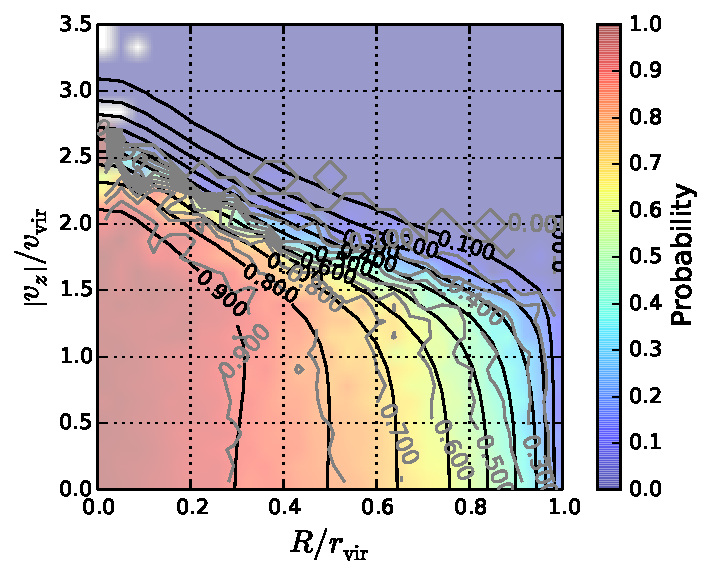
\includegraphics[width=0.6\linewidth]{figures/maggie/probabilities.pdf}
    \caption{Contours of halo membership probability from the simulation of
        \citet{Borgani+01} as stacked by~\cite{MBM+10} and our model. In
        \emph{gray} the contours obtained with particles from the cosmological
        simulation, and in \emph{black} the theoretical expectation from
        \bartrefequation{gi_over_gh}. The color scale reflects the probability
        from the simulation. The theoretical probability agrees with the
        cosmological simulation except for high velocities along the
    line-of-sight.\label{fig:probabilities}}
\end{figure}

\remark{%
    We may think that the observed discrepancies in
    \bartreffigure{probabilities} are the consequence of a bad choice for the
    ratio of anisotropy radius to scale radius $b/a$ (see
    \bartrefappendix{profiles}) or for the concentration, but changing this
    value doesn't reduce them. The contours for the simulation seem to show a
    cut-off in the line-of-sight velocity dispersion for high velocities, as
    if the distribution is truncated above a given velocity. A functional form
    with such a property is the generalization of the Gaussian called the
    $q$-Gaussian or Tsallis distribution. Assuming such a velocity
    distribution, the computation of the probability involves several
    integrals, which is CPU time consuming. Instead, we can fit a $q$-Gaussian
    on the line-of-sight velocity distribution from the simulation and
    incorporate it in the probability computation. But unfortunately, this
    doesn't solve the problem. It seems that the number of particles with high
    velocities is too low to correctly define the probability to be in the
    virial sphere of the halo, and to compare it to theoretical expectations.
    The velocity distribution isn't involved.
}

Here, we assume that an NFW density profile, since the dark matter particles of
the \citet{Borgani+04} simulation follow this distribution (see~\cite{MBM+10}).
But we are interested in groups of galaxies and they must follow the same
distribution to apply our model. We used the galaxies from the $z=0$ output of
the \citet{Guo+11} semi-analytical code and checked that they follow a NFW
density profile too. But as expected, there is a bias between the galaxies and
dark matter particles. Indeed, if we fit the concentration of the NFW profile
in \citet{Guo+11} and compare it to the model of \citet{Maccio+08} obtained
from dark matter particles, we can see that the two functions are different. A
consequence is that the link between halo mass and concentration must be
adjusted for galaxies in our model. The difference between the two
concentration-mass relations is shown in \bartreffigure{concentration_bias}.
%
\begin{figure}[ht]
    \centering
    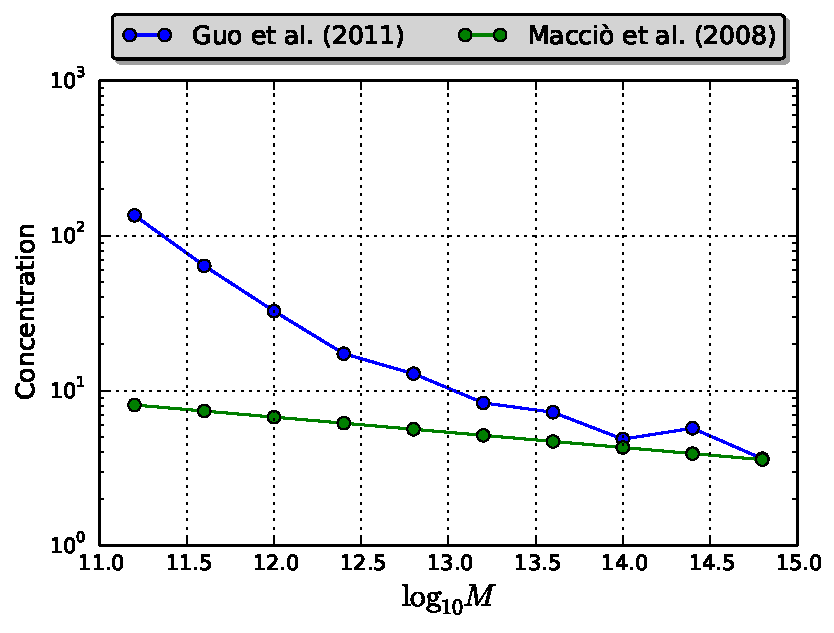
\includegraphics[width=0.8\linewidth]{figures/maggie/concentrations.pdf}
    \caption{halo concentration as a function of halo mass for
        \citet{Maccio+08} in \emph{green} and concentration of the galaxy
        population (NFW fit) from \citet{Guo+11} with $M_r\leqslant-15$ in
        \emph{blue}. In low mass halos, the concentration of galaxies is much
    higher than that of dark matter particles.\label{fig:concentration_bias}}
\end{figure}
%
But we note that the modulation of the concentration with the halo mass is
dependent of the cut-off in luminosity applied to the galaxy sample, making the
use of a specific density profile for galaxies inadequate. We checked the
influence of this choice on MAGGIE by comparing the performance with the
concentration from \citet{Guo+11} and from \citet{Maccio+08}. No noticeable
impact is observed in the completeness, reliability and fragmentation, except
on stellar masses and luminosities of groups but without being significant.

\section{Results on mock catalogues}
\label{sec:results_on_mock_catalogue}

\subsection{Description}
\label{sub:maggie_tests_description}

For tests, we proceed as described in \citet{Yang+07, Duarte+14} and
\bartrefchapter{friends_of_friends_algorithm}. To link a selected group by the
algorithm in redshift space to the true halo in real space, we use the most
massive galaxy of the group. The true halo of a group is the true halo to which
the most massive galaxy in the selected group (referred as the central galaxy)
belongs to. With this link, we compute the completeness and reliability of
groups relatively to this halo in real space. We define statistics used to
quantify the performance of MAGGIE\@. The completeness $C$ is the fraction of
galaxies in the real space group (limited to the virial sphere) recovered in
the selected group. The reliability $R$ is the fraction of galaxies in the
selected group present in the real space group (limited again to the virial
sphere). A primary group is defined as a selected group whose central galaxy
matches the central galaxy of the real space associated group, remaining groups
are fragments. A complete and detailed description of the statistics can be
found in \citet{Duarte+14} and \bartrefchapter{friends_of_friends_algorithm}.

The reliability in the case of MAGGIE is more complex since we use
probabilities for galaxies in groups. To take advantage of our probabilities,
let us give a new definition for the reliability. In \citet{Duarte+14}, we
wrote:
%
\begin{equation}
    R=\frac{\mathrm{TG} \cap \mathrm{EG}}{\mathrm{EG}}=
    \frac{\sum_{i\in \mathrm{TG}\cap \mathrm{EG}}}{\sum_{i\in \mathrm{EG}}}
\end{equation}
%
But many galaxies belong to our group with this definition and so we
weight galaxies in the previous sum by their probabilities in order to have
a coherent definition of the reliability with our probabilistic
determination of groups. Our new definition in the case of a probabilistic
galaxy group algorithm as MAGGIE is:
%
\begin{equation}
    R=\frac{\mathrm{TG} \cap \mathrm{EG}}{\mathrm{EG}}=
    \frac{\sum_{i\in \mathrm{TG}\cap \mathrm{EG}} p_i}
    {\sum_{i\in \mathrm{EG}}p_i}
\end{equation}
%
For the completeness, since the probability doesn't introduce a bias in the
selection relatively to the real group, we keep the computation as described
in \citet{Duarte+14}, without weighting by probabilities.

Without probabilities, galaxies in groups form a complete partition of the
survey since groups can be seen as disjoints sets of redshift space. But with
MAGGIE and probabilities, a galaxy can be in multiple groups so the sets of
groups are overlapping, and the \emph{dual} analysis in \citet{Duarte+14} for
the merging of real space groups cannot be correctly done. This is because the
central galaxy of a real space group can potentially belong to several
extracted groups in redshift space.

\subsection{Optimization}

MAGGIE depends on two probability thresholds: the first we call central
probability ($p_\mathrm{cen}$) constraining the fragmentation of galaxy groups
by allowing galaxies to be the central galaxy of a potential galaxy group, the
second one the membership probability ($p_\mathrm{mem}$), defining a threshold
to consider or not a galaxy in a group for the computation of its properties.

In fact, a galaxy is considered as possible central galaxy while looping
through ordered galaxies only if the galaxy has all its probabilities in its
other groups lower than the central probability threshold. For membership,
galaxies are ``assigned'' to a group (i.e.\ they are assumed to have a
probability to be in this group) only if their probabilities are above the
threshold membership probability.

Checking the dependence of MAGGIE to these parameters is done in the same way
as we performed in \bartrefchapter{friends_of_friends_algorithm}. We computed
the mean completeness, reliability, fragmentation and merging, as well as the
quality factors we previously defined, for a range of threshold probabilities
$(p_\mathrm{central}, p_\mathrm{membership})\in{\left[10^{-15}, 0.4\right]}^2$.
Fortunately, results are not dependent on these thresholds. A small variation
is observed only for very high values of these probabilities (above 0.1).
Increasing these probabilities leads to relatively worst statistics, while
keeping them small is better, but without significant variations.

We selected $p_\mathrm{cen}=p_\mathrm{mem}=0.001$. Since this value is
relatively small, we should notice that it is equivalent to defining the
membership in the virial cone constructed with the virial radius of the group.
The selection of background galaxies, far away in velocities, is avoided by
$p_\mathrm{mem}$, since with these value, when galaxies are beyond than
4--5 $\vvir$ from the group, they are not considered. The same happens
for $p_\mathrm{cen}$ where galaxies in membership can't create new groups.

When working with non-probabilistic algorithms, the set of galaxy groups is a
complete partition of the space formed by galaxies. In other words, groups are
non-overlapping and fragmentation is avoided naturally if the assignment is
done properly. But with probabilities and our method, removing these threshold
parameters, there are as many groups as galaxies. Setting the two thresholds to
zero makes MAGGIE behave like non-probabilistic algorithms. Note that if we set
$p_\mathrm{mem}=0$, each galaxy group will be formed of its entire virial cone,
which is not desirable. The introduction of threshold probabilities is a way to
make a ``compatibility'' between MAGGIE with its soft assignment and
non-probabilistic grouping algorithms and their hard assignments.

\subsection{Results}

The following tests result from the application of MAGGIE on the perfect (no
observational errors, no K-corrections) mock catalogue whose construction is
described in \bartrefchapter{mock}. In this case, we assume the halo mass
function extracted from the Millennium-II outputs, with an NFW galaxy number
density profile identical to that for dark matter particles in their halos. The
influence of these assumptions will be developed in
\bartrefsection{maggie_discussions}, in particular the incorporation of
observational errors in our mocks.

We compare MAGGIE with the popular FoF grouping algorithm (see
\bartrefchapter{friends_of_friends_algorithm}). The set of linking lengths used
for the FoF is the one defined in~\cite{Duarte+14} for an optimal FoF, close to
the parameters used by~\cite{Robotham+11}, with values of (\bperp,
\bpar)$=(0.07, 1.1)$. This will let us see if the our probabilistic Bayesian
approach improves the galaxy grouping compared to a simple geometrical approach
such as FoF.

\subsubsection{Fragmentation}

Estimating the fraction of groups in the selection that are the result of the
fragmentation of a real group is important since an observer using a group
catalog can't distinguish the primary group from the other. In
\bartreffigure{fragments}, we show the fraction of fragmented groups (defined
as in \bartrefchapter{friends_of_friends_algorithm}) as a function of the
estimated group mass. This allows to see the expected fraction of fragmented
groups by an observer using a group catalog with only information on the
estimated halo mass.

MAGGIE shows much less fragmentation than FoF, for all estimated group masses,
such $\log_{10} M/M_\odot \geqslant 12$ (nearby sample) or $12.3$ (distant
sample). This is due to the combination of the
abundance matching that gives good estimates of group virial masses and the ordered
search of groups from galaxy stellar masses. But fragmentation increases
with the decreasing estimated mass, since with groups of few members, it
is easier to make a mistake in the selection of the central galaxy of the
group.

\subsubsection{Completeness and reliability}

\begin{figure}[t]
    \centering
    \begin{minipage}{0.49\linewidth}
        \subfloat[Catalogue 2]
        {%
            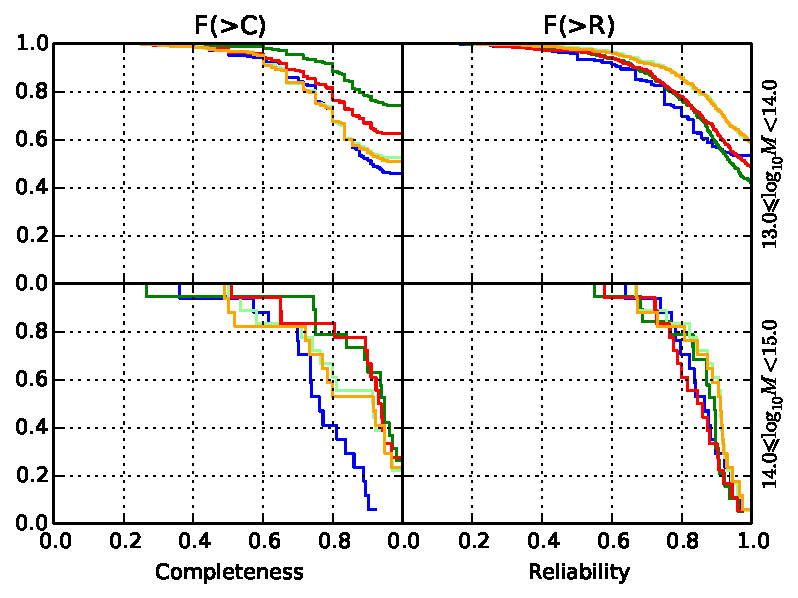
\includegraphics[width=\linewidth]{%
figures/maggie/article_fof_comparison_errors_CDF_completeness_reliability_1_article_C_R.pdf%
            }
        }
    \end{minipage}
    \begin{minipage}{0.49\linewidth}
        \subfloat[Catalogue 5]
        {%
            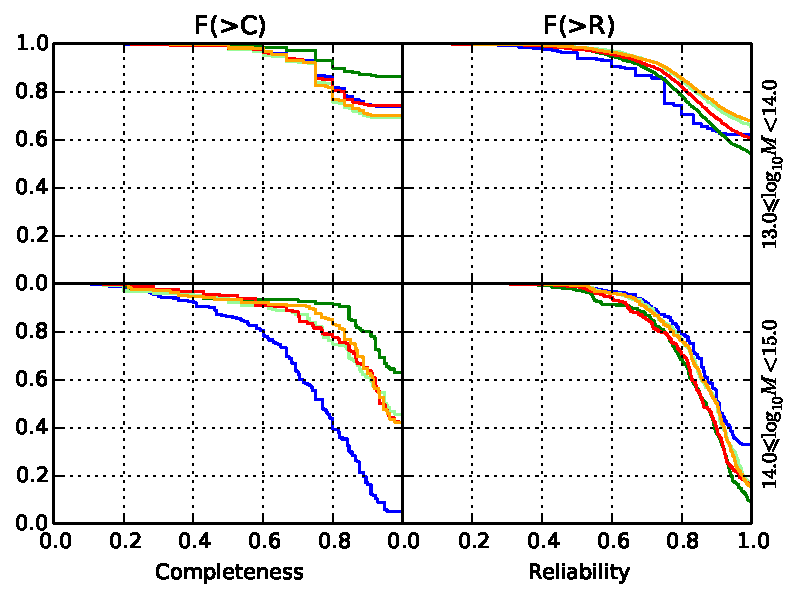
\includegraphics[width=\linewidth]{%
figures/maggie/article_fof_comparison_errors_CDF_completeness_reliability_4_article_C_R.pdf%
            }
        }
    \end{minipage}
    \caption{The cumulative distribution functions of the completeness $F(>C)$
        and reliability $F(>R)$ for bins of true halo mass for two sub-samples
        of the mock catalogue (nearby in left and distant in right). The
        colored histograms are for FoF (\emph{blue}), MAGGIE-m with no
        observational errors (\emph{dark green}), MAGGIE-L with no
        observational errors (\emph{light green}), MAGGIE-m with $0.2$ dex
        errors on stellar mass (\emph{red}) and MAGGIE-L with $0.04$ dex errors
        on luminosites (\emph{gold}). Details for
        latter cases are in \bartrefsubsection{observational_errors}. Results
        are shown only for primary groups (i.e.\ groups that are not fragments
    of real space halos) with the same filter as in
\bartrefchapter{friends_of_friends_algorithm}.\label{fig:comp_rel}}
\end{figure}

\bartreffigure{comp_rel} shows the cumulative distribution functions of the
completeness $C$ and reliability $R$ as defined in
\bartrefsubsection{maggie_tests_description} for MAGGIE and the FoF algorithm.
Results are shown only for two doubly complete sub-samples (see
\bartrefchapter{mock}), different with
\bartrefchapter{friends_of_friends_algorithm}, where we use now catalogues 2
and 5. Only two bins in true group virial halo mass are used. MAGGIE (in dark
green) shows a better behaviour in completeness for all masses in both
catalogues than FoF (in blue), while the reliability is equivalent to the
optimal FoF, except for high masses for the more distant catalogue, where FoF
is more reliable (median reliability is $0.90$ for FoF and $0.85$ for MAGGIE).

\subsubsection{Virial masses}
%
\begin{figure}[htb]
    \centering
    \begin{minipage}{0.39\linewidth}
        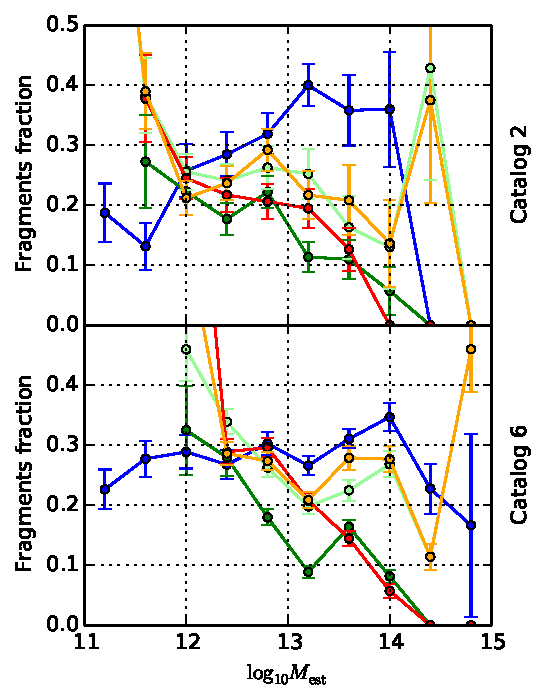
\includegraphics[width=\linewidth]{%
    figures/maggie/article_fof_comparison_errors_frag_fraction_fragments.pdf%
        }
        \captionof{figure}{The fraction of estimated groups that are fragments
        in bins of estimated mass of extracted groups, for catalogues 2 and 5.
    Colors are the same as in \bartreffigure{comp_rel}.\label{fig:fragments}}
    \end{minipage}
    \begin{minipage}{0.6\linewidth}
        \centering
        \begin{minipage}{\linewidth}
            \subfloat[Comparison of virial masses]
            {%
                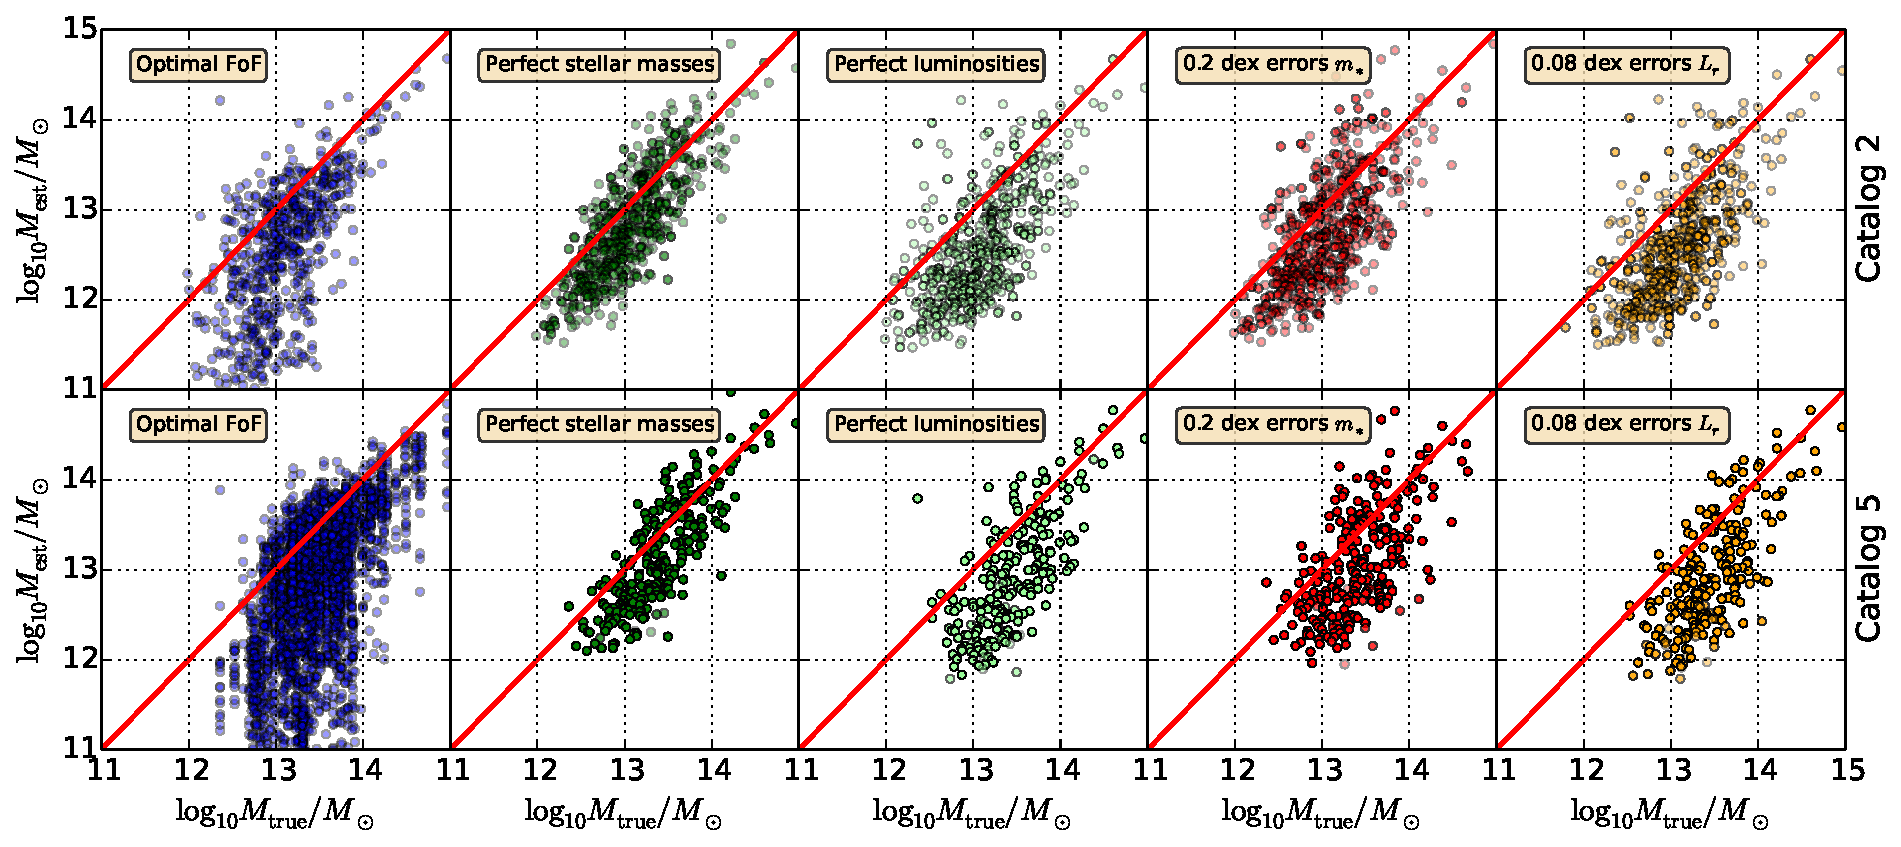
\includegraphics[width=\linewidth]{%
        figures/maggie/article_fof_comparison_errors_differences_halo_mass.pdf%
                }
            }
        \end{minipage}
        \begin{minipage}{\linewidth}
            \subfloat[Bias and dispersion for virial masses]
            {%
                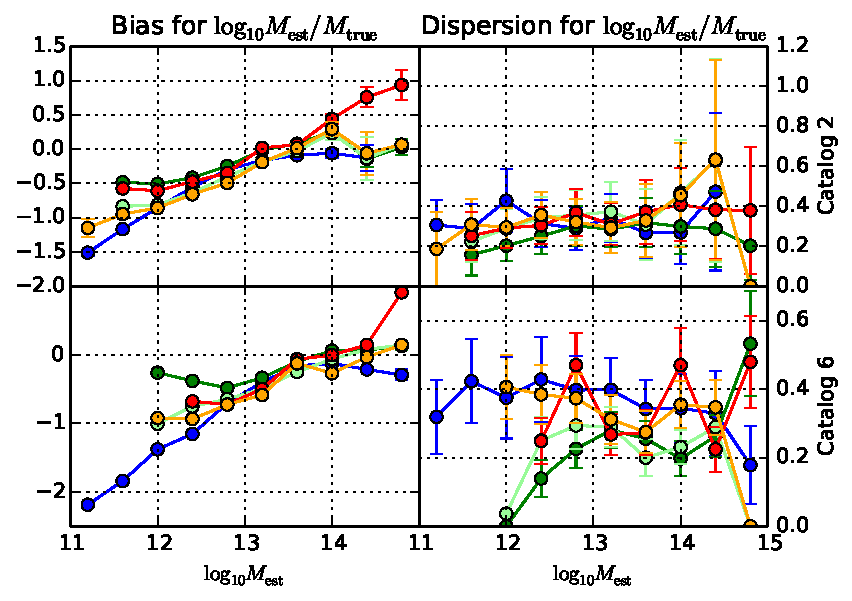
\includegraphics[width=\linewidth]{%
    figures/maggie/article_fof_comparison_errors_bias_dispersion_halo_mass.pdf%
                }
            }
        \end{minipage}
        \captionof{figure}{Comparison of the virial mass estimated by the
            galaxy group algorithms and the true masses obtained from the
            Millennium-II simulation, for catalogues 2 and 5. The top panel
            shows the comparison and the bottom panel bias and the dispersion
            of the logarithmic difference of masses. Colors are the same as in
        \bartreffigure{comp_rel}.\label{fig:bias_disp_virial_mass}}
    \end{minipage}
\end{figure}

In the \bartreffigure{bias_disp_virial_mass}, we compare the estimation of the
virial mass by application of the virial theorem for FoF algorithm and by
abundance matching for MAGGIE\@. As we already discussed, the virial theorem
isn't very suitable in recovering the virial masses of groups when they have a
small mass (between $10^{12}$ and $10^{13}M_\odot$). We can't really see this
in the bias of the estimation between the two algorithms. On the other hand,
the scatter in recovered masses of groups in the distant sub-sample is lower
with MAGGIE (0.25 dex) than with FoF (0.35 dex), except for
$M\geqslant10^{15}M_\odot$, where MAGGIE suffers from uncertainties in the
abundance matching caused by small number statistics at the high end. In the
nearby sub-sample, both MAGGIE and FoF produce scatter in virial mass of
$\approx 0.3$ dex.

\subsubsection{Group luminosities and stellar masses}

\begin{figure}[htb]
    \centering
    \begin{minipage}{\linewidth}
        \centering
        \subfloat[Comparison for group luminosities]
        {%
            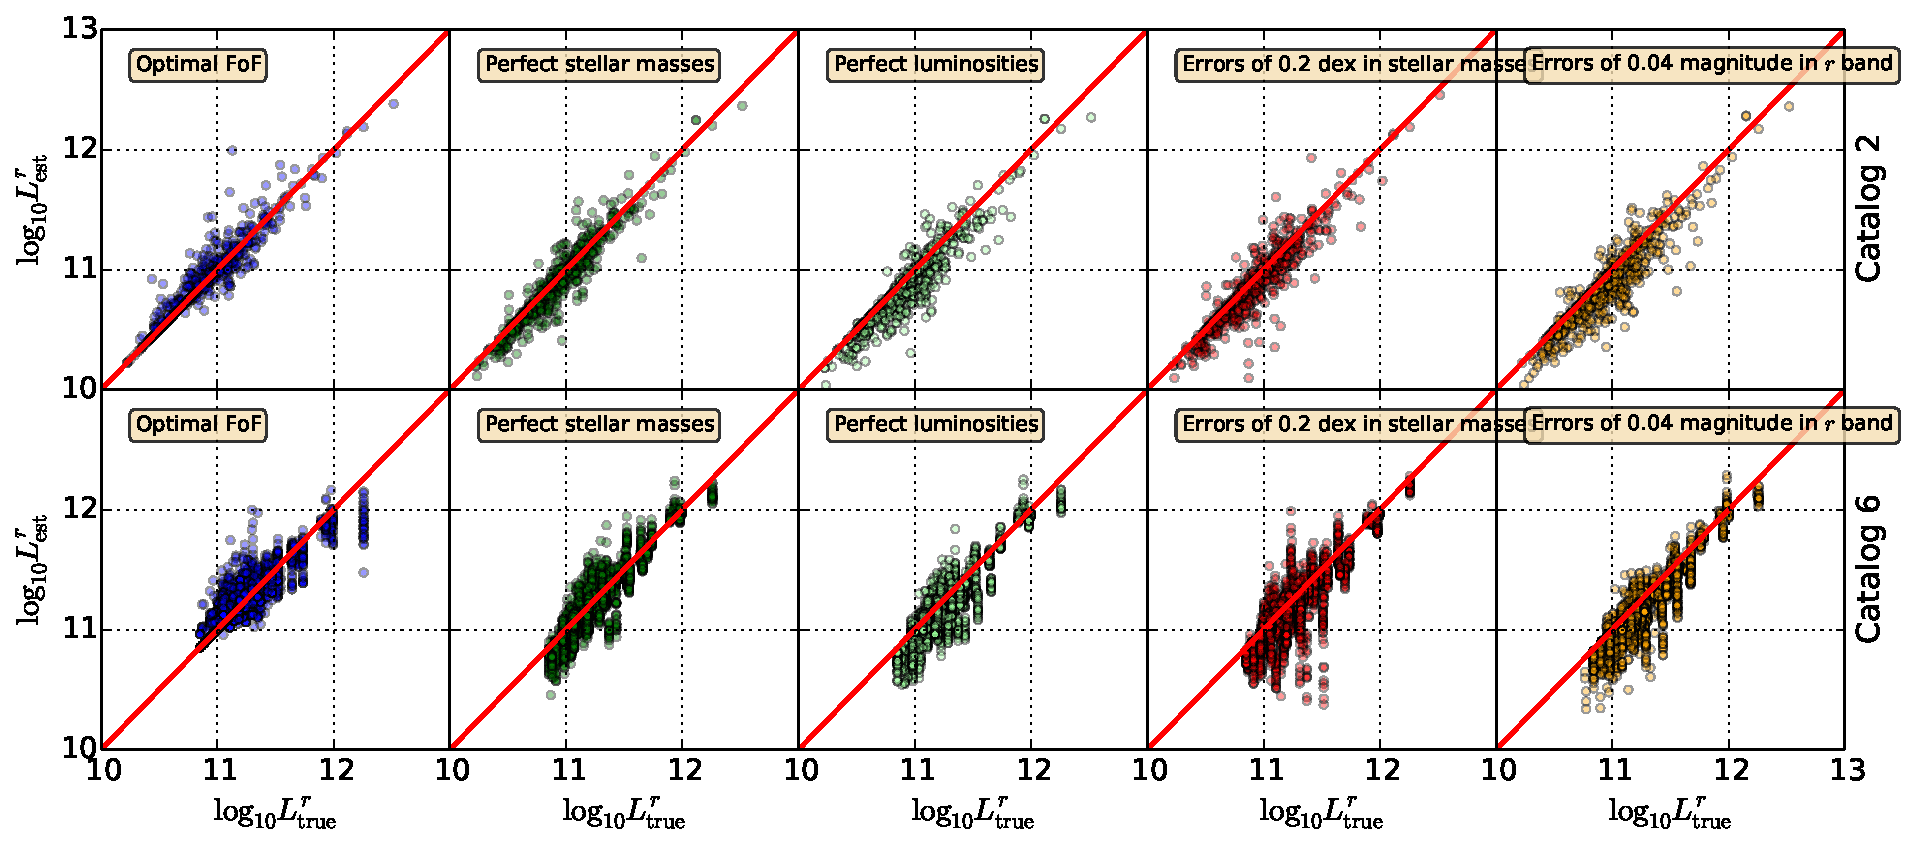
\includegraphics[width=0.8\linewidth]{%
figures/maggie/article_fof_comparison_errors_differences_luminosity.pdf%
            }
        }
    \end{minipage}
    \begin{minipage}{\linewidth}
        \centering
        \subfloat[Comparison for group stellar masses]
        {%
            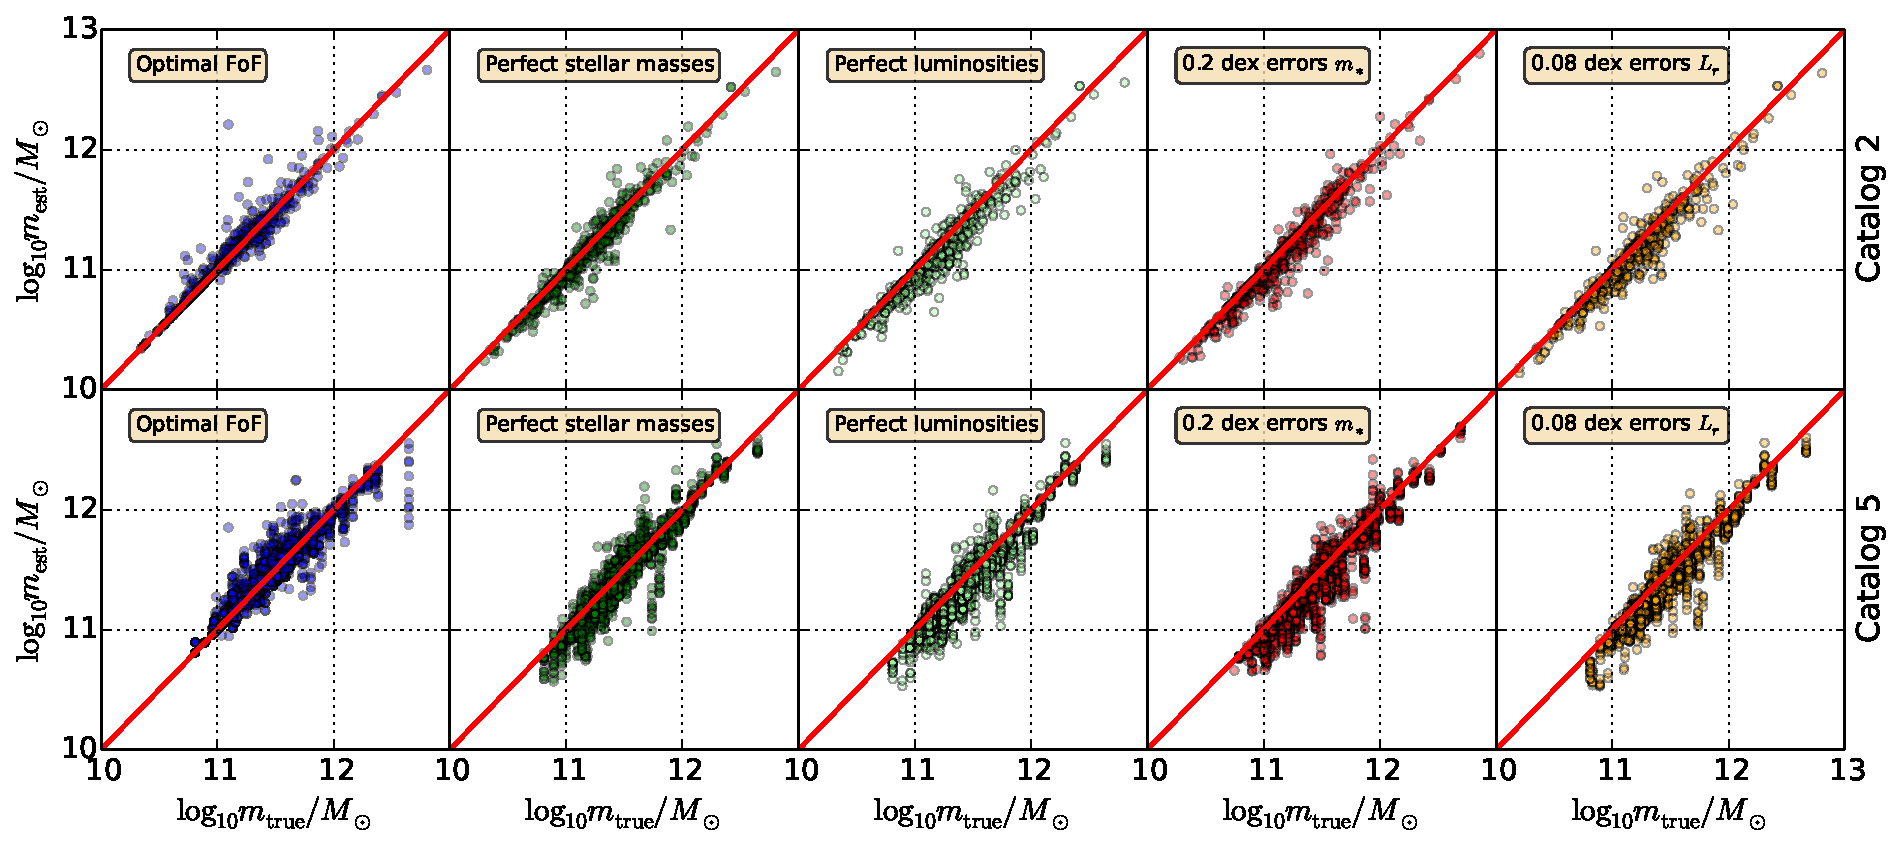
\includegraphics[width=0.8\linewidth]{%
figures/maggie/article_fof_comparison_errors_differences_stellarmass.pdf%
            }
        }
    \end{minipage}
    \captionof{figure}{Comparison of group luminosities in $r$ band and stellar
    masses with the real space for primary groups in catalogues 2 and
5.\label{fig:comparison}. Colors are the same as in \bartreffigure{comp_rel}.}
\end{figure}
%
\begin{figure}[htb]
    \centering
    \begin{minipage}{0.49\linewidth}
        \centering
        \subfloat[Bias and dispersion for luminosities]
        {%
            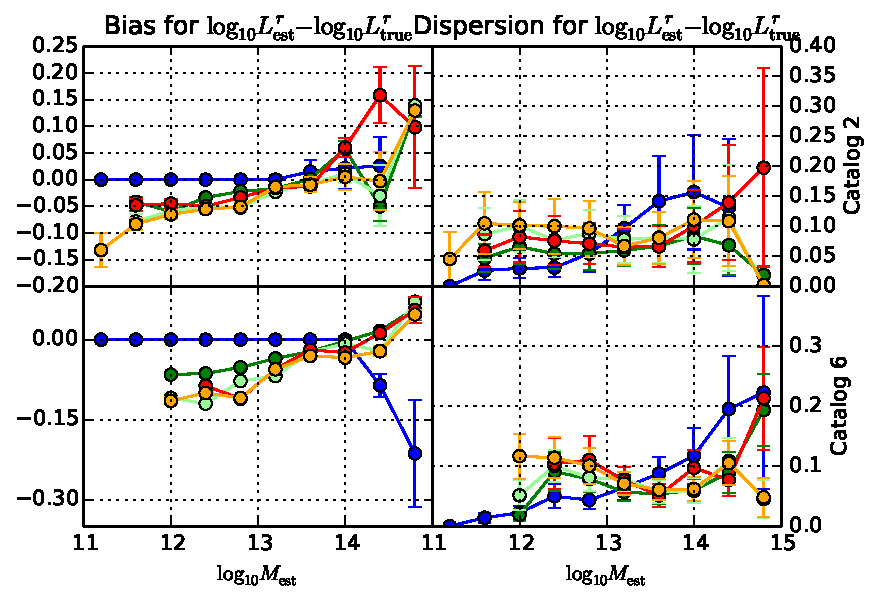
\includegraphics[width=\linewidth]{%
figures/maggie/article_fof_comparison_errors_bias_dispersion_luminosity.pdf%
            }
        }
    \end{minipage}
    \begin{minipage}{0.49\linewidth}
        \centering
        \subfloat[Bias and dispersion for stellar masses]
        {%
            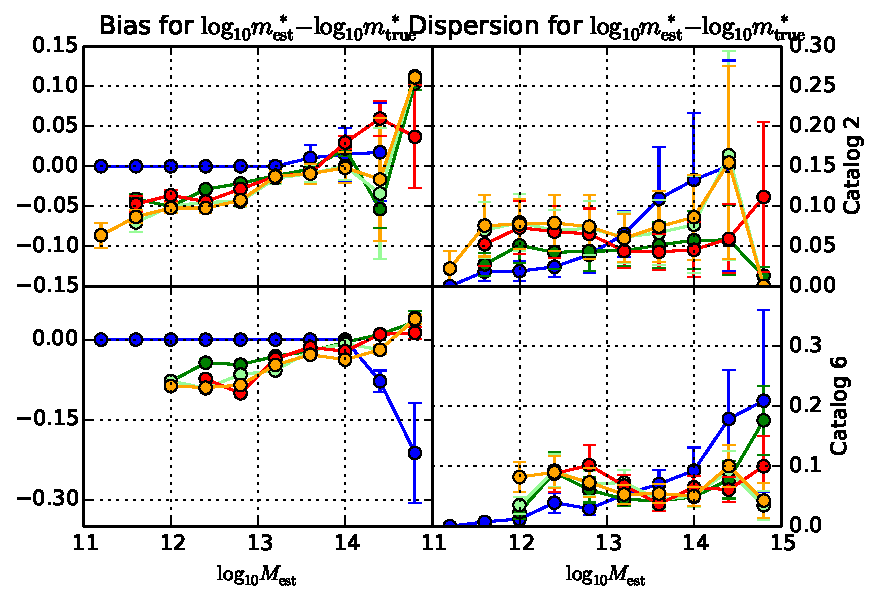
\includegraphics[width=\linewidth]{%
figures/maggie/article_fof_comparison_errors_bias_dispersion_stellarmass_bias.pdf%
            }
        }
    \end{minipage}
    \captionof{figure}{Bias and dispersion for group luminosities and stellar
    masses for catalogues 2 and 5. Colors are the same as in
\bartreffigure{comp_rel}.\label{fig:bias_disp}}
\end{figure}

We test the deduced stellar mass and luminosity of selected groups for each
algorithm. For non-probabilistic FoF, they are just the sum of the galaxy
contributions. But for MAGGIE, we use the computed probabilities inside the
group to weight the stellar mass and luminosity of each galaxy. If $X$ is the
property of the group, $x_i$ the property of the galaxy $i$ in the group with
the probability $p_i$:
%
\begin{equation}
    X = \sum_i p_i x_i
\end{equation}

In \bartreffigure{comparison} and \bartreffigure{bias_disp}, we compare the
true luminosity of groups (computed assuming a perfect selection of groups in
the sub-sample) with the luminosity computed with the galaxy membership of each
algorithm. In the bottom panel, we show the bias and the dispersion of the
difference between the true and estimated luminosities. These figures show the
same for stellar masses. The optimal FoF algorithm has a lower bias than MAGGIE
since we can't observe a trend of the bias with the true halo mass, while the
scatter is lower for MAGGIE at high masses ($13.3\leqslant
\log_{10}M/M_\odot\leqslant 14.7$) thanks to the probability weighting that
reduces the effect of interlopers.

\section{Discussions}
\label{sec:maggie_discussions}

A simple comparison of MAGGIE with the most popular and geometrical grouping
algorithm shows that MAGGIE is well adapted in recovering galaxy groups from
redshift space catalogues. Extracted global properties of groups are less
biased and catastrophic cases avoided by using probabilities as weights to
smooth the estimation. The membership inside these groups is better too since
the completeness shows that MAGGIE selects a large part of galaxies from the
real group, without polluting it by interlopers (as shown by the reliability).
Moreover, the importance of interlopers is reduced still by using
probabilities. The abundance matching technique is also a very good way to
contribute to this galaxy group extraction, since the virial mass estimation
relies only on group or galaxy properties, which are observables certainly
biased and uncertain, but with less importance than biased geometrical
informations (velocity dispersion, richness\ldots). On the contrary, a
geometrical based group finder such as FoF performs well when the number of
galaxies is important because interlopers act as a small noise in the group
membership, even with their relatively important presence at high halo masses
for the FoF algorithm. Hence, velocity dispersion and harmonic radius are more
efficient with high richness and the virial theorem thus becomes more precise.

This comparison is done in the case where the data on galaxies is perfect, in
the sense that there are no observational errors and we perfectly know the
various scaling relations used in our models. But the behaviour of MAGGIE is
unknown in the real situation of an observer, with a limited knowledge in these
models. In the following sections, we study the robustness of the performance
of MAGGIE under pertubations, i.e.\ in cases where we modify our initial
estimate of virial radius, aw well as the halo mass function, and when we take
into account observational errors in the galaxy luminosities and stellar
masses.

\subsection{Prior halo mass --- central stellar mass relation}
\label{sub:prior_relation}

We tested the choice for the initial relation between the halo mass and the
central stellar mass of groups to see its effects on MAGGIE\@. We used the
relation from \citet{BCW+10} against a simple ratio relation with different
values for the ratio. Extracted groups are insensitive to this choice, if we
keep this choice with physical values. The iterative process corrects a bad
assumption in our initial guess.

\subsection{Influence of the halo mass function model}
\label{sub:hmf_test}

The estimation of the virial mass (radius) is a crucial step of MAGGIE (and
other Bayesian methods). A biased estimate of group masses will affect observed
trends of galaxy properties with the global environment.

Our mass computation needs to be precise in the largest mass range possible,
and independent of the pollution of groups by interlopers. The abundance
matching technique seems to be a good way to estimate the virial mass of galaxy
group halos. In principle, it seems more biased than using the luminosities or
stellar masses of groups, but since the central galaxy in a selected group is
well recovered, this is a quantity less affected by interlopers and so the halo
mass estimation will be good enough. But since there is a saturation of the
relation between the halo mass and the central stellar mass at high halo mass,
we expect that the estimation will be poorer for high masses than other
methods.

Most halo mass functions described in the literature fit the FoF mass of the
halos instead of the spherical over-density mass, which is related to the
virial mass of the halo. Since we used the galaxy catalogue from
\citet{Guo+11}, whose semi-analytical code was applied onto the Millennium-II
run, we fit the virial halo mass function directly on its output. We show it in
\bartreffigure{hmf} where we plot the FoF mass function (in red) and the virial
mass function (in black) for halos in the Millennium-II simulations at redshift
zero. Virial masses are lower than FoF masses so we don't use existing models
of halo mass functions displayed too on the figure. The way of computing such
halo mass functions is described in \bartrefappendix{halo_mass_functions}.

\begin{figure}[htbp]
    \centering
    \begin{minipage}{0.49\linewidth}
        \subfloat[Catalogue 2]{%
            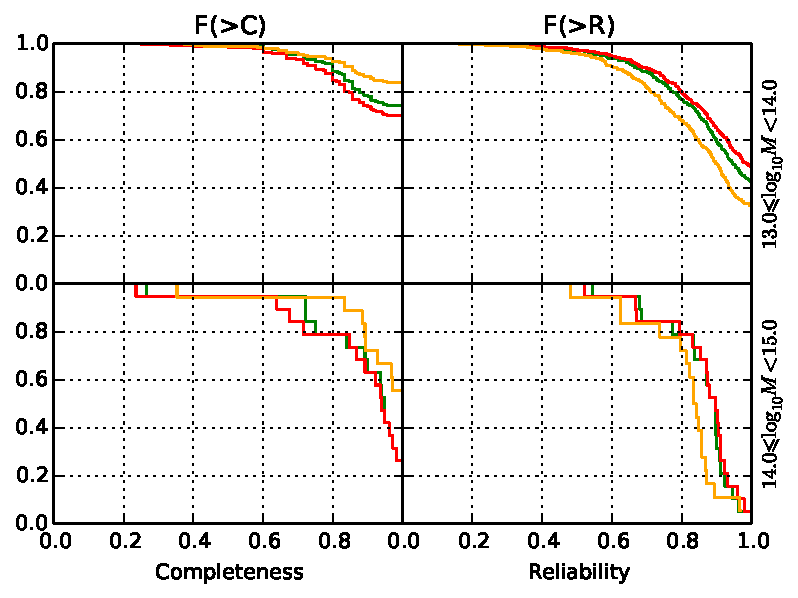
\includegraphics[width=\linewidth]{%
figures/maggie/msii_courtin_warren_CDF_completeness_reliability_1_article_C_R.pdf%
            }
        }
    \end{minipage}
    \begin{minipage}{0.49\linewidth}
        \subfloat[Catalogue 5]{%
            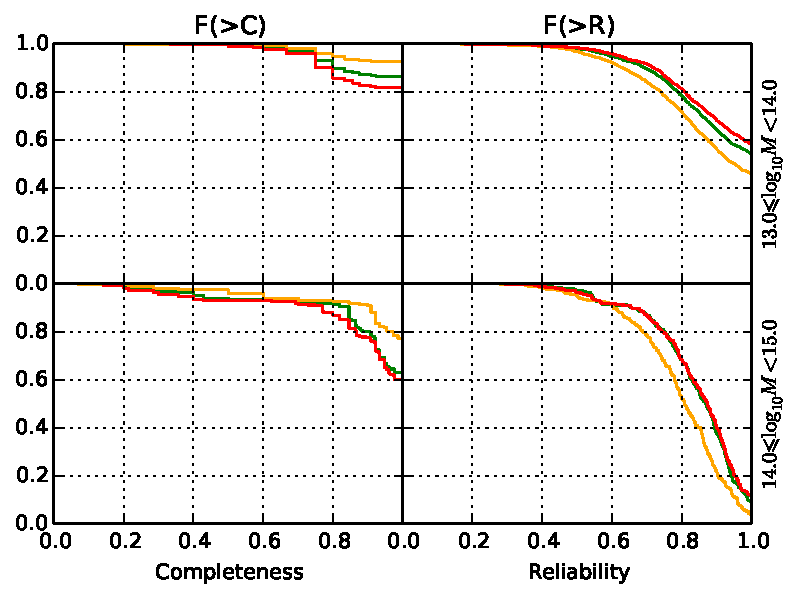
\includegraphics[width=\linewidth]{%
figures/maggie/msii_courtin_warren_CDF_completeness_reliability_4_article_C_R.pdf%
            }
        }
    \end{minipage}
    \captionof{figure}{The cumulative distribution functions of the
        completeness and reliability for comparison of the perfect case of
        MAGGIE-m in \emph{green} with the halo mass function model
        of~\cite{Warren+06} in \emph{orange} and~\cite{Courtin+11} in
    \emph{red}. The filter applied on groups is the same as in
\bartrefchapter{friends_of_friends_algorithm}. The three different halo mass
functions lead to similar group memberships.\label{fig:cdf_hmf}}
\end{figure}
%
\begin{figure}[htbp]
    \centering
    \begin{minipage}{0.49\linewidth}
        \subfloat[Group halo masses]{%
            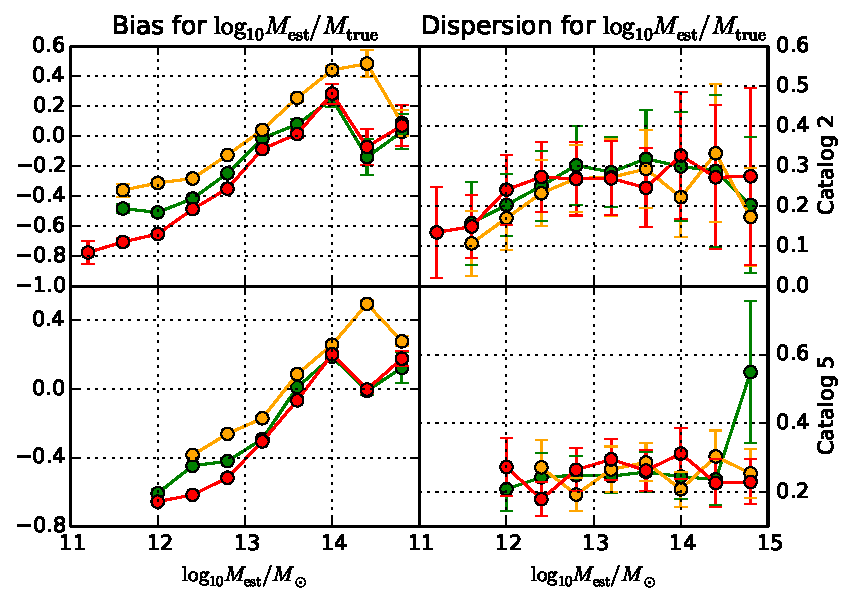
\includegraphics[width=\linewidth]{%
        figures/maggie/msii_courtin_warren_bias_dispersion_halo_mass.pdf%
            }
        }
    \end{minipage}
    \begin{minipage}{0.49\linewidth}
        \subfloat[Group stellar masses]{%
            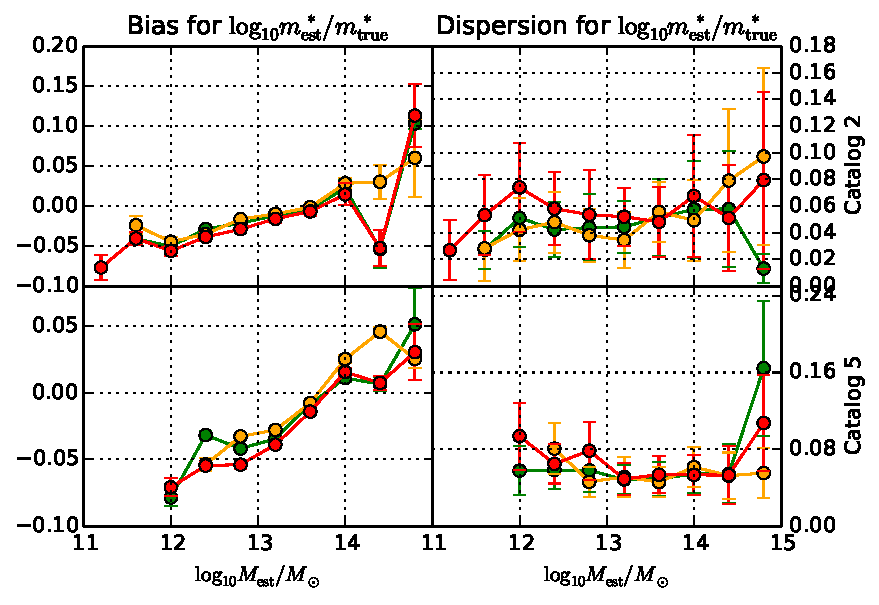
\includegraphics[width=\linewidth]{%
    figures/maggie/msii_courtin_warren_bias_dispersion_stellarmass_bias.pdf%
            }
        }
    \end{minipage}
    \begin{minipage}{0.49\linewidth}
        \subfloat[Group luminosities]{%
            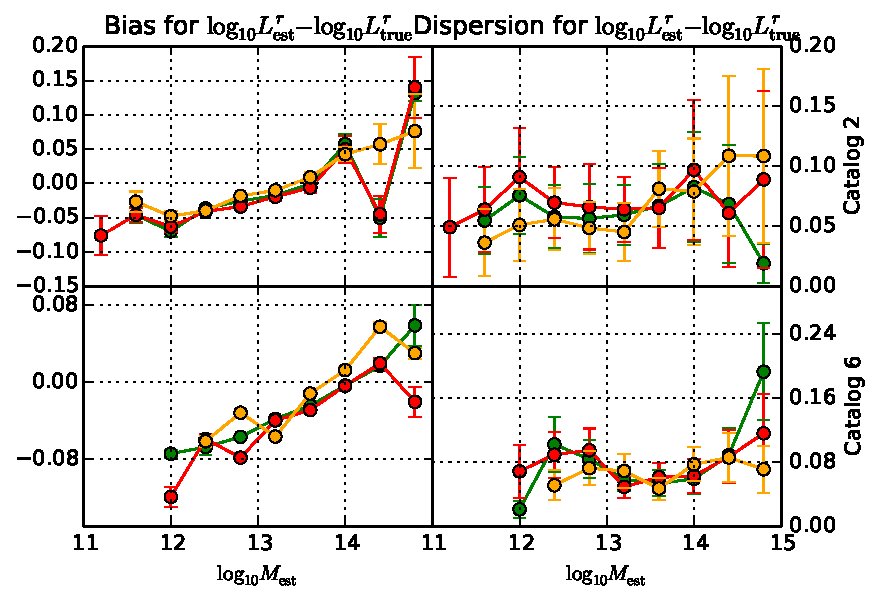
\includegraphics[width=\linewidth]{%
        figures/maggie/msii_courtin_warren_bias_dispersion_luminosity.pdf%
            }
        }
    \end{minipage}
    \captionof{figure}{Group properties compared to the perfect case of
        MAGGIE-m (no observational errors) using the halo mass function
        measured in the Millennium-II output, for both~\cite{Warren+06}
        and~\cite{Courtin+11} halo mass functions. Colors and filter are the
    same as in \bartreffigure{cdf_hmf}. As seen in \bartreffigure{cdf_hmf},
differences are not really significant.\label{fig:bias_disp_hmf}}
\end{figure}

The robustness of MAGGIE against the choice of the halo mass function is
important because this choice will affect the completeness and reliability of
our selected groups and their properties too in a non obvious way. Indeed, the
halo mass function is a prior in MAGGIE and doesn't reflect necessary the
reality. We apply an equivalent of the perturbation method to test the
stability of MAGGIE under a bad choice of model. We used two halo mass
functions very different of the halo mass function measured on the
Millennium-II simulation: \citet{Warren+06} and \citet{Courtin+11}. Those
models are fits of the FoF halo mass function from different cosmological
simulations. This is not the same as the virial mass but ideal for a
perturbation test. The result of the application of MAGGIE with these models is
shown in \bartreffigure{cdf_hmf} and \bartreffigure{bias_disp_hmf}.

Comparisons are performed against the perfect case of MAGGIE-m (no
observational errors) in green with the halo mass function directly fitted on
the Millennium-II, perfect stellar masses and luminosities for galaxies. In
orange, halo mass function of \citet{Warren+06} and in red, that one of
\citet{Courtin+11}. The influence of the halo mass function is very small on
the completeness and reliability for all catalogues and for group properties.
The fragmentation is not shown but behaves like in other plots, not affected by
the choice of halo mass function.

\subsection{Influence of cosmological parameters}

Our problematic is still the same: as an observer, we don't know the real space
and its properties. So, we assume a given set of cosmological parameters. When
applying group finders on our mock catalog, we use the cosmology of the
simulation from which are constructed our mock. But in reality, we know those
parameters with a given uncertainty and we want to know their effects on the
group extraction.

To answer this question, we must know where the cosmology is relevant in the
algorithm. For example, when computing the projected radius of a galaxy at the
redshift of the group, we implicitly need to compute the luminosity distance
which is cosmology dependent. We assume in our case a flat Universe and in this
case, it is computed using just elliptic integrals
\citep{Liu+11,Eisenstein+97}. So cosmological parameters have an influence on
this distance, and in consequence, on the membership of galaxy groups.
Moreover, the halo mass function is dependent of the cosmology assumed by the
observer for many models and can affect the virial mass estimations. In our
case, the halo mass function is fitted on the real space data and its influence
can't be really measured. But we expect it has the same influence as a bad
choice for the halo mass function. We ran MAGGIE with the true cosmology (from
Millennium-II simulation) and two false cosmology with respect to our mock
catalog (Planck and WMAP9) to compare results. As expected, the importance of
the cosmology is low, of the order of statistical errors, as seen in
\bartreffigure{cdf_cosmology} and \bartreffigure{bias_disp_cosmology}.
%
\begin{figure}[htbp]
    \centering
    \begin{minipage}{\linewidth}
        \centering
        \begin{minipage}{0.49\linewidth}
            \subfloat[Catalogue 2]{%
                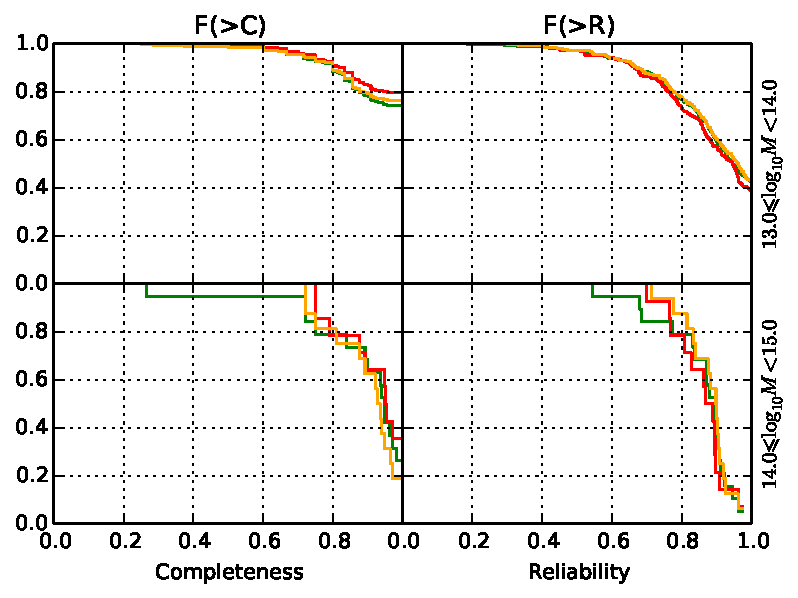
\includegraphics[width=\linewidth]{%
figures/maggie/planck_wmap9_CDF_completeness_reliability_1_article_C_R.pdf%
                }
            }
        \end{minipage}
        \begin{minipage}{0.49\linewidth}
            \subfloat[Catalogue 5]{%
                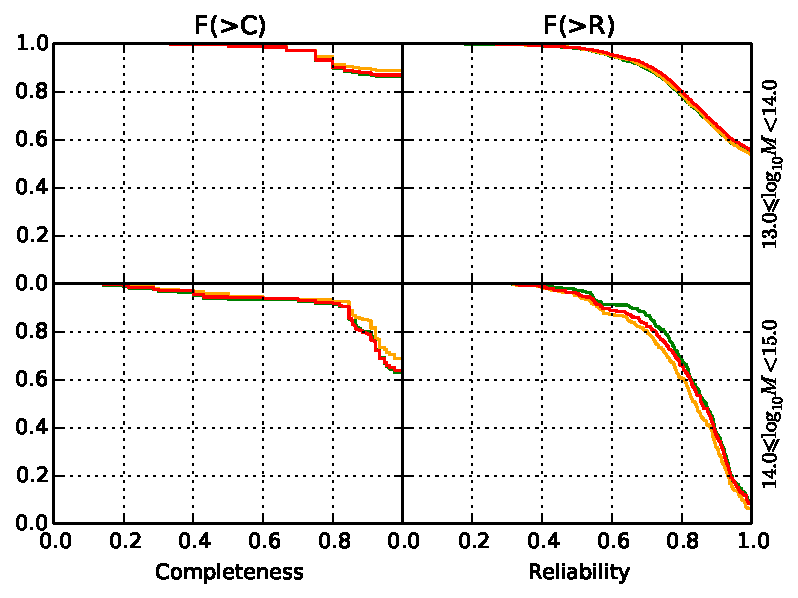
\includegraphics[width=\linewidth]{%
figures/maggie/planck_wmap9_CDF_completeness_reliability_4_article_C_R.pdf%
                }
            }
        \end{minipage}
    \captionof{figure}{The cumulative distribution functions of the
        completeness and reliability for comparison of the perfect case of
        MAGGIE-m (no observational errors) (\emph{green}) to different
        cosmologies \emph{orange} for~\cite{PlanckXVI} and \emph{red}
    for~\cite{Bennett+13}. Errors in the cosmological parameters don't have a
significant impact on the group extraction.\label{fig:cdf_cosmology}}
    \end{minipage}
    \begin{minipage}{\linewidth}
        \centering
        \begin{minipage}{0.49\linewidth}
            \subfloat[Group halo masses]{%
                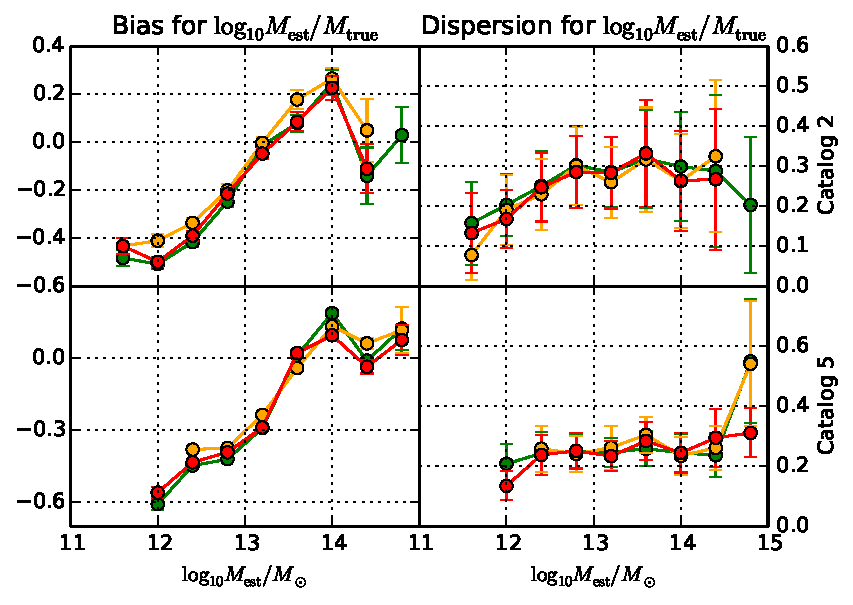
\includegraphics[width=\linewidth]{%
                figures/maggie/planck_wmap9_bias_dispersion_halo_mass.pdf%
                }
            }
        \end{minipage}
        \begin{minipage}{0.49\linewidth}
            \subfloat[Group stellar masses]{%
                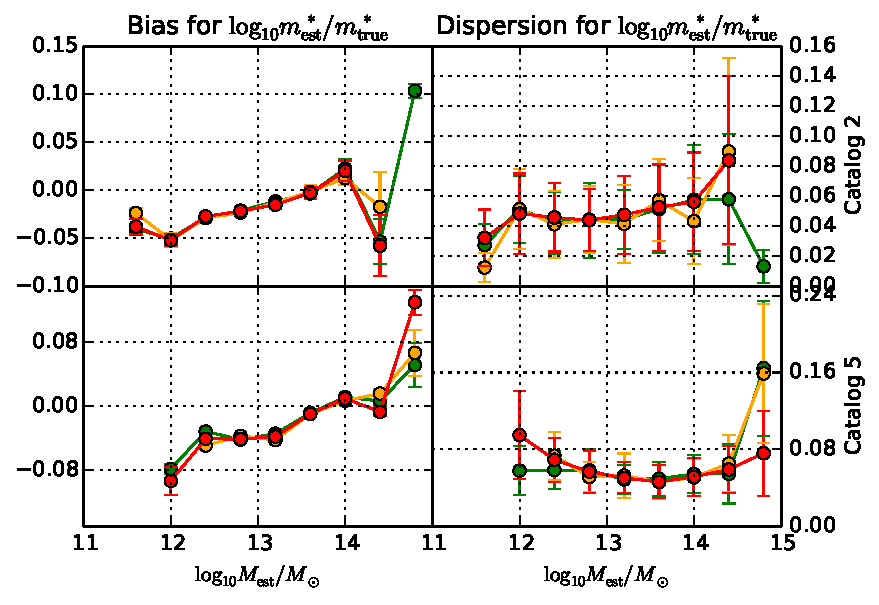
\includegraphics[width=\linewidth]{%
            figures/maggie/planck_wmap9_bias_dispersion_stellarmass_bias.pdf%
                }
            }
        \end{minipage}
        \begin{minipage}{0.49\linewidth}
            \subfloat[Group luminosities]{%
                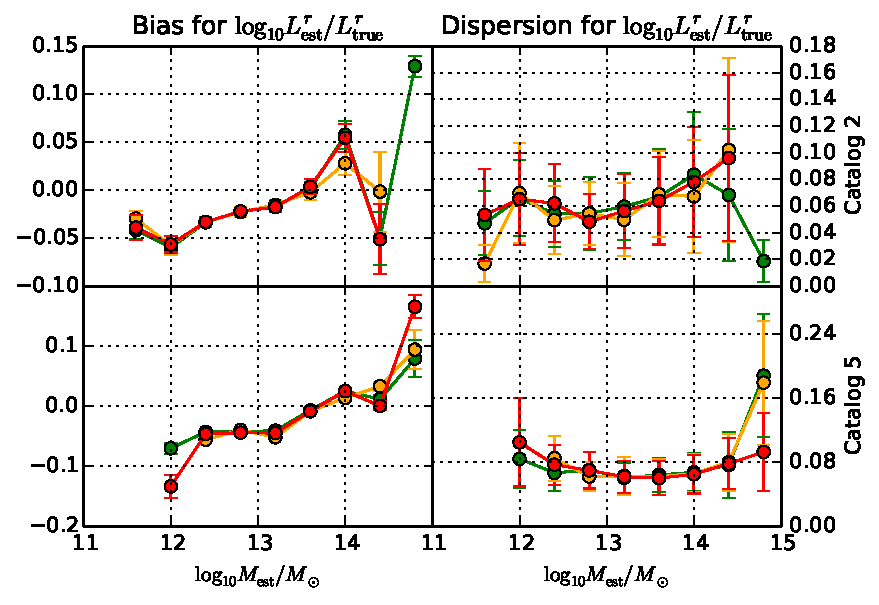
\includegraphics[width=\linewidth]{%
                figures/maggie/planck_wmap9_bias_dispersion_luminosity.pdf%
                }
            }
        \end{minipage}
        \captionof{figure}{Group properties compared to the perfect case (no
            observational errors) of MAGGIE-m for both~\cite{PlanckXVI}
            and~\cite{Bennett+13} cosmologies. Colors are the same as in
            \bartreffigure{cdf_cosmology}. Again, the differences are not
        significant.\label{fig:bias_disp_cosmology}}
    \end{minipage}
\end{figure}

\subsection{Influence of observational errors}
\label{sub:observational_errors}

Our way of sorting galaxies by mass uses our prior on the galaxy formation
scenario. Indeed, the stellar mass of the central galaxy of a dark matter halo
is correlated to its virial mass. But the relation is saturated at high halo
masses. So the intrinsic precision is affected by this choice. Moreover, the
estimation of stellar masses from the observations and spectrum is not very
precise and can significantly differ according to the way of computing it. We
show the differences between several spectral models present in the SDSS data
base, with the bias and dispersion for each distribution, in
\bartrefchapter{sdss}.

Typically, the errors in the estimation of stellar mass is roughly 0.2 dex. We
introduce such errors in the stellar masses of the mock catalogue to estimate
the effect of the bad estimation. We generated Gaussian errors without bias and
dispersion of 0.2 dex. The application of MAGGIE-m on these galaxy mock
catalogues is shown on \bartreffigure{comp_rel}, \bartreffigure{comparison},
\bartreffigure{bias_disp}, \bartreffigure{fragments} and
\bartreffigure{bias_disp_virial_mass} in red.

The effect of an error on stellar masses is quite catastrophic in the
completeness, compared to the case where the stellar masses are perfect (in
green). The percentage of groups with a perfect completeness decreases for
around 20 points for the catalogue 5 with a large volume, while this effect
isn't visible in the catalog 2 for high mass halos (since the volume of the
catalog is smaller, the number of high halo mass we expect to find is small too
and statistics poorer). The effect on the reliability is less important since
probabilities reduce the importance of interlopers introduced by the decrease
in completeness. In contrary, galaxy group properties are not very affected by
these errors in stellar masses, except for high halo masses. In this case, if
the most massive galaxy has not its mass well estimated, the estimation of the
halo mass is bad and probabilities can't ``correct'' this effect properly. This
is visible in \bartreffigure{bias_disp_virial_mass} where the bias in the
estimation of the halo mass is very important for high halo masses and the
dispersion is increased in all range of masses. In the other hand, the
fragmentation is increased for smaller halo masses, since with the decline in
completeness due to errors, high mass halos decompose into smaller parts at the
origin of the observed fragments.

So, errors in stellar masses are problematic and we should use an other tracer
for the halo mass as the central luminosity, which is less affected by
observational errors. Indeed, the principal sources of errors in the
computation of the absolute magnitude of a galaxy are the photometry, the
extinction, the K-correction, and the redshift through the distance modulus:
%
\begin{equation} \Delta M=\Delta m + \frac{5}{\ln{10}} \frac{\Delta
d_\mathrm{lum} \left(z\right)}{\Delta z} \frac{1}{d_\mathrm{lum}
\left(z\right)} + \Delta E + \Delta K\left(z\right) \end{equation}
%
$\Delta m$ for apparent magnitudes is of the order of $10^{-2}$ in the SDSS,
the second term is between $10^{-4}$ and $10^{-2}$ in the range of redshift
used for the catalogues. The K-correction $\Delta K$, if we follow the method
of \citet{Chilingarian+10}, is of the order of $10^{-2}$. There is the problem
of the extinction $\Delta E$ for which the precision can't be really estimated.
The Galactic extinction is estimated to 0.075, but the internal extinction of
galaxies is more imprecise and we provide a rough value of 0.1. Moreover,
peculiar velocities worst the situation since they contribute to the
computation of the distance modulus. But for non-nearby galaxies and globally,
the errors should be small.

The inclusion of the luminosity instead of stellar mass in the group extraction
process of MAGGIE is quite simple. The abundance matching between the virial
mass and the central stellar mass is replaced by an abundance matching between
the virial mass and the central luminosity. Intrinsically, using luminosities
instead of stellar masses in the inference of group virial masses is expected
to be less precise because the relation between the luminosity of the central
galaxy and the halo mass is more saturated for high mass groups. But the gain
is in the precision and the robustness relatively to the precision.

Comparing the perfect case of MAGGIE using galaxy luminosity (light green) to
the perfect case of stellar masses (dark green) shows, as expected, that the
completeness is worst for luminosities (the reliability is a little better
since the completeness has decreased). But group properties are not really
affected still by the use of probabilities to avoid bad membership. The
fragmentation is worst too since groups aren't entirely recovered (missing
galaxies are considered as belonging to fragment groups). For halo mass
estimations, the bias induced by using luminosities is comparable to the
perfect case of stellar masses. It is only in the dispersion that we observe
the counterparts, specifically for high halo masses, due to the uncertainties
introduced by the saturation in the relation between the central luminosity and
the virial mass in this range of halo masses. But it is approximately better
than using stellar masses with errors.

Adding errors following a Gaussian distribution without bias and a dispersion
of 0.08 dex on luminosities (0.2 magnitudes as we roughly deduced previously),
we compare it (light orange) to the perfect case of the luminosity. As
expected, introduced errors doesn't have a real impact, because the behaviour
of light orange and light green curves are roughly identical.

The negative point of using luminosities instead of stellar masses is that it
seems to increase the fragmentation of true groups. But this fragmentation
remains lower than that found for the FoF group. We should discuss a little how
we make a match between the real space and the observed space. To say which
galaxy is the central of a group in the real space, we can't directly use the
one given by~\cite{Guo+11} since in our mock catalogue, there is a magnitude
limit removing a large number of galaxies not sufficiently luminous. The
central is not necessarily the most luminous of the group and the flux limit
can possibly hide us the central while the group is visible with help of some
of its galaxies. To define the central galaxy in real space, we use the most
massive in stellar mass of the group taking into account only galaxies within
the complete sample used. Without such a treatment, we could possibly increase
the fragmentation artificially by a lack of central galaxy in the sample. With
MAGGIE-L, the central galaxy in extracted groups has a strong chance to be the
most luminous (not necessarily the most massive in stellar mass) and the match
with real space groups will frequently say that the central galaxy of the
extracted group is not the same as the true group, resulting in a frequent
fragmentation in our tests. This is what we observe in the results of MAGGIE-L.

A possible conclusion is that observational errors are very important when
working with Bayesian galaxy group algorithms based on physical priors,
contrary to geometrical based algorithms, where such uncertainties do not
influence their performances.

\subsection{Conclusion}
\label{sub:maggie_discussion_conclusion}

MAGGIE performs quite well in comparison to the optimal FoF. The use of
probabilities to recover group properties is very useful to reduce the effect
of inevitable interlopers present in the group membership. But when applied on
data with uncertainties, its performances are reduced compared to tests with a
perfect knowledge of the various needed observables. Although there are some
counterparts for MAGGIE on realistic data, we note that globally it performs
better than the FoF algorithm applied on perfect data. The extracted membership
is better than the FoF and the virial mass estimation by abundance matching
compared to the simple virial theorem used generally with FoF.

This makes MAGGIE a suitable grouping algorithm to be applied on large
galaxy surveys such as the Sloan Digital Sky Survey (SDSS) and the Galaxy And
Mass Assembly (GAMA).

% vim: set tw=79 ft=tex:
